\subsection{Descripci\'on del problema}

En este ejercicio se nos presenta el juego Roban\'umeros, un juego de dos jugadores que consiste en lo siguiente:

\begin{itemize}
\item Se juega con cartas y cada una tiene un n\'umero entero
\item Se juega por turnos alternados entre ambos jugadores. Un jugador no puede elegir pasar, es decir que debe jugar en todos sus turnos
\item Al comenzar el juego se pone sobre la mesa una secuencia de cartas boca arriba, la cantidad puede ser cualquiera
\item En su turno el jugador puede tomar la cantidad de cartas que quiera. Las cartas tomadas deben ser adyacentes y el jugador puede elegir de qu\'e extremo sacarlas (izquierda o derecha). 
\item El juego termina cuando se terminan las cartas
\item Gana el jugador que sume m\'as puntos con las cartas que tom\'o
\end{itemize}

Un ejemplo de la disposici\'on inicial de las cartas puede ser el siguiente:\\

\begin{figure}[h]
\begin{center}
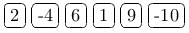
\includegraphics[scale=0.6]{./img/ej1_explicacion1.png}
\caption{Caso ejemplo}
\end{center}
\end{figure}

En este caso, un jugador podr\'ia robar las cartas 2, -4 y 6 o -10, 9, 1, 6, pero no 2, 6, 9 ya que no son adyacentes. \\

Para este caso en particular el juego se desarrollar\'ia de la siguiente manera:

\begin{itemize}
\item Mingo toma 5 cartas desde la izquierda (2, -4, 6, 1 y 9) sumando 14 puntos.
\item An\'ibal toma la \'unica carta restante, el -10.
\end{itemize}

El juego lo gana Mingo logrando una diferencia de 24 puntos.

\subsection{Resoluci\'on}

Para resolver el problema $P$ dado de longitud $n$ cartas, debemos construir una funcion $F$ tal que F(P[0..n-1]) este definida como "La jugada que logre la mejor diferencia con el oponente, sabiendo que el mismo juega de forma \'optima" \\

Pensando de manera mas precisa la funci\'on, podriamos escribirla como: \\

F(P[0..n-1]) = MAX(Tomar una carta desde la izquierda y restarle F(P[1..n-1]), Tomar dos cartas desde la izquierda y restarle F(P[2..n-1]), ..., Tomar todas las cartas, ... , Tomar n-2 cartas desde la derecha y restarte F(P[0..0])) \\

Como podemos ver, habr\'ia que tomar la m\'axima diferencia de puntos obtenidos entre las cartas que uno toma y las que toma el oponente, que como sabemos juega de manera \'optima (como nosotros), por eso evaluamos la misma funci\'on para el pero sin las cartas que ya tomamos nosotros. \\

Definamos esta funci\'on recursivamente (usamos una funcion $h$ para lograr claridad): \\

$
F(P) =
\left\{
	\begin{array}{ll}
		P_{0}  & \mbox{if } |P| = 1 \\
		max( h_{izq} (0, n), ... , h_{izq} (k, n) , ... , \sum\limits_{i=0}^n P_{i} , h_{der} (n-1, n), ... , h_{der} (k, n) , ... )  & \mbox{if } |P| > 1
	\end{array}
\right.
$ \\

Las funciones $h_{izq}$ y $h_{der}$ devuelven la diferencia de una jugada en particular tomando una cantidad de cartas y restandole el puntaje del rival con las cartas restantes: \\

$h_{izq}(fin, n) =  (\sum\limits_{i=0}^{fin} P_{i}) - F(P[fin+1...n-1])$ \\
$h_{der}(inicio, n) =  (\sum\limits_{i=inicio}^{n-1} P_{i}) - F(P[0...inicio-1])$\\

La funci\'on F genera un arbol con todas las posibilidades y finalmente nos devuelve la mejor diferencia posible. Como podemos ver en el ejemplo esta clase de problemas tiene solapamiento de subproblemas, por lo cual una versi\'on recursiva a secas no es la manera \'optima de implementar la soluci\'on. 

\begin{figure}[h]
\begin{center}
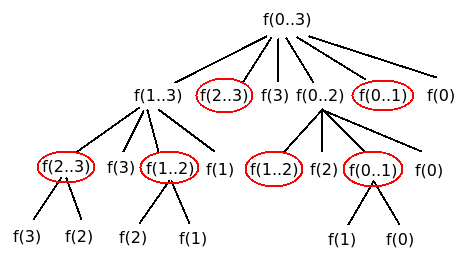
\includegraphics[scale=0.6]{./img/ej1_res1.png}
\caption{\'Arbol representativo de la funci\'on recursiva con los subproblemas requeridos para cada problema en particular, en rojo se marcan los subproblemas solapados}
\end{center}
\end{figure}

\subsection{Demostraci\'on de la resoluci\'on}

\subsection{Complejidad del algoritmo}

\subsection{C\'odigo fuente}

\subsection{Casos de prueba}

\subsection{Performance}
